% ==========================================================================
\section{Computer Operation}
% ==========================================================================

    % ==========================================================================
    \subsection{ON/OFF button}
    % ==========================================================================
    \label{subsec:onoffbutt}

    The ON/OFF button is located on the lefthand side of the back of the
    computer.

    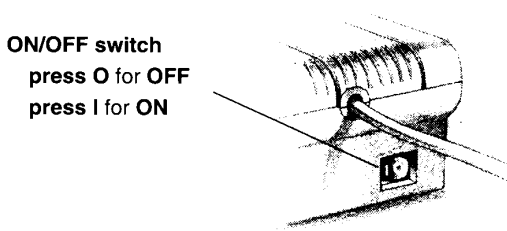
\includegraphics[scale=0.5]{images/onoffbutton.png}

    This button is used to turn ON and OFF the computer.

    Before turning it ON, read the instriuctions on the section
    \hyperref[sec:setting_system]{Setting up the system} of this manual.

    Before turning it OFF, it is highly recommended to use the command 
    \hyperref[cmd:halt]{halt} to ensure that all \textbf{DISK} data has been
    correctly saved. Otherwise, corruption of data may occur.

    % ==========================================================================
    \subsection{Reset button}
    % ==========================================================================
    \label{subsec:resetbutton}

    The reset button is located on the lefthand side of the computer.

    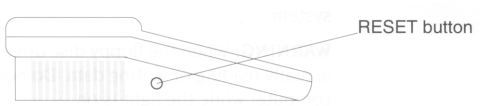
\includegraphics[scale=0.7]{images/resetbutton.png}

    This button is used to restart the computer without turning it off via the
    \hyperref[subsec:onoffbutt]{ON/OFF button}.

    To reset the computer simply press and release the button. The reset process
    will take 6.5 seconds in total, as explained in the section
    \textit{Reset circuit} of the dastaZ80 Technical Reference
    Manual\cite{dastaz80techman}.

    % ==========================================================================
    \subsection{Indicator LEDs}
    % ==========================================================================

    At the top of the computer case there a few labelled LEDs\footnote{A
    Light-Emitting Diode (LED) is a semiconductor device that emits light when
    current flows through it.} that give information of the status of several
    internal parts of the computer.

    \begin{itemize}
        \item Above the numeric pad, on the righthand side of the keyboard,
        there are two LEDs:
        \begin{itemize}
            \item \textbf{POWER}. This LED is always on when the computer is
            switched on via the \hyperref[subsec:onoffbutt]{ON/OFF button}. It glows
            in \underline{orange} colour.
            \item \textbf{DISC}. This LED blinks whenever a \textbf{DISK} operation
            (read/write) is happening. It glows in \underline{green} colour.
        \end{itemize}
    \end{itemize}
    
    \centerline{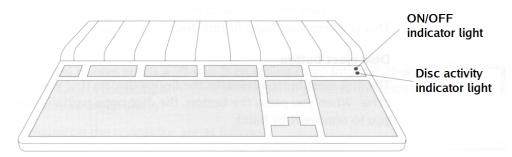
\includegraphics[scale=0.5]{images/keyboardLEDs.png}}

    \begin{itemize}
        \item Above the \textit{Esc} and function keys (\textit{F1}-\textit{F12}),
        on the lefthand side of the keyboard, there are two LEDs. These LEDs are
        multi-colour, hence glowing at different colour each:
        \begin{itemize}
            \item Computer status
            \begin{itemize}
                \item \textbf{RESET}. It glows in \underline{red} colour when
                the computer is in reset status. This happens for 6.5 seconds
                when the computer is switched ON (via the
                \hyperref[subsec:onoffbutt]{ON/OFF button}) and when the
                computer is reset via the \hyperref[subsec:resetbutton]
                {Reset button}.
                \item \textbf{HALTED}. It glows in \underline{blue} when the
                computer is in halt status. Usually after issuing the command
                \hyperref[cmd:halt]{halt}.
                \item \textbf{ROM PAGED}. It glows in \underline{green} when the
                \textbf{ROM} has been electrically disconnected and therefore
                the computer will only perform operations (read/write) from/to
                the \textbf{RAM}. This happens only during the Boot Sequence.
                See the section \textit{OS Boot Sequence} of the dastaZ80
                Programmer's Reference Guide\cite{dastaz80progref} for more
                detailed information about the Boot Sequence.
            \end{itemize}
            \item Clock Selection
            \begin{itemize}
                \item \textbf{CLOCKSEL}. It glows in \underline{yellow} colour
                when the Internal clock is used. And in \underline{purple}
                colour when an External clock is being used by the computer.
            \end{itemize}
        \end{itemize}
    \end{itemize}

    % ==========================================================================
    \subsubsection{MicroSD}
    % ==========================================================================

    At the back of the computer there is a MicroSD slot.

    Insert here a MicroSD formatted with FAT32 and containing Disk Image
    Files formatted with DZFS\footnote{DZFS (dastaZ80 File System) is a file
    system of my own design, for mass storage devices, aimed at simplicity}.

    \centerline{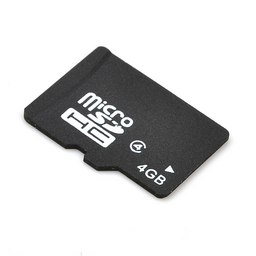
\includegraphics[scale=0.5]{images/microsdcard.png}}

    % ==========================================================================
    \subsection{3.5 inch Floppy Disc Drive}
    % ==========================================================================

    The Floppy Disc Drive is located on the righthand side of the computer.

    3.5 inch floppy discs can be inserted in this drive. 

    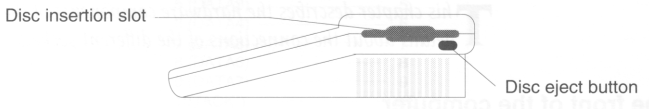
\includegraphics[scale=0.7]{images/discslot.png}

    To remove an inserted floppy disc from the drive, press the
    \textit{Disc eject button}. The disc will partially pop out, allowing you to
    completelly remove it by hand.

    % ==========================================================================
    \subsection{Attaching peripheral devices}
    % ==========================================================================

        % ==========================================================================
        \subsubsection{Dual Video Output}
        % ==========================================================================

        At the back of the computer you will find two connectors, beside each
        other, for the connection of video output.

        The first one, and necessary to use the computer, is a VGA connector for
        the \textbf{VGA video output}.
        
        Plug here a standard VGA cable connected to a VGA monitor.

        \centerline{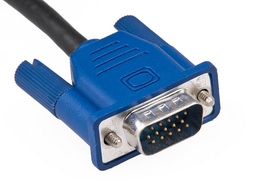
\includegraphics[scale=0.5]{images/vgaconn.png}}

        The second connector, which is optional (i.e. the computer will function
        perfectly normal without this connected), is a 3.5mm female jack for the
        \textbf{Composite video output}\footnote{The Composite video signal is
        NTSC (National Television System Committee), the standard for analog
        television used mainly in USA, Japan and some parts of South America}.

        Plug here the jack side of a 3.5mm jack-to-3-RCA Audio/Video cable
        \footnote{This is the same cable used on the Raspberry Pi for Composite
        output.}.

        \centerline{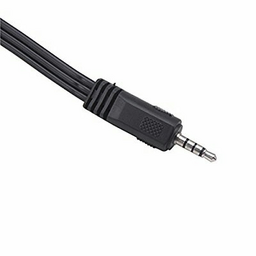
\includegraphics[scale=0.5]{images/raspicable_jack.png}}

        Connect the yellow RCA cable of the jack-to-3-RCA cable to the Composite
        input of a monitor or TV.

        \centerline{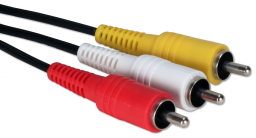
\includegraphics[scale=0.5]{images/raspicable_rca.png}}

        % ==========================================================================
        \subsubsection{Stereo Sound Output}
        % ==========================================================================

        The stereo sound signal comes out of the same connector used for the
        Composite video output.

        Connect the jack-to-3-RCA white and red cables to a pair of speakers or
        to the input of a sound system amplifier.

        % ==========================================================================
        \subsubsection{USB Keyboard for External computer}
        % ==========================================================================

        The keyboard of the dastaZ80 can be used as an USB keyboard on other
        computers.
        
        Connect the a USB cable between this connector and your other
        computer, switch on dastaZ80 and press the key \textit{ScrollLock}. From
        now on (as indicated by the ScrollLock LED being lighted) dastaZ80 will
        not read any keystrokes, but instead will send them to the computer
        connected via USB.

        If you want to use dastaZ80 at any time, just press \textit{ScrollLock}
        again. There is no need to unplug the USB cable. The \textit{ScrollLock}
        key is doing the switching.

        This feature can be handy when you are using dastaZ80 and another PC at
        the same time and don't want to be switching hands between two keyboards
        all the time. It saves space too!

        % ==========================================================================
        \subsubsection{ROM Cartridge}
        % ==========================================================================

        Refer to the section \textit{Cartridge Port} of the dastaZ80 Technical
        Reference Manual\cite{dastaz80techman} for more detailed information.

        % % ==========================================================================
        % \subsubsection{General-Purpose Input/Output (GPIO)}
        % % ==========================================================================

        % This connector exposes all CPU signals and can be used to connect external
        % devices directly to the components (e.g. \textbf{CPU}, \textbf{RAM)} of
        % the computer.